\documentclass[12pt,a4paper]{article}
\usepackage{ctex}
\usepackage{amsmath,amscd,amsbsy,amssymb,latexsym,url,bm,amsthm,float}
\usepackage{epsfig,graphicx,subfigure}
\usepackage{enumitem,balance}
\usepackage{wrapfig}
\usepackage{mathrsfs,euscript}
\usepackage[usenames]{xcolor}
\usepackage{hyperref}
\usepackage[vlined,ruled,linesnumbered]{algorithm2e}
\usepackage{array}
\hypersetup{colorlinks=true,linkcolor=black}

\newtheorem{theorem}{Theorem}
\newtheorem{lemma}[theorem]{Lemma}
\newtheorem{proposition}[theorem]{Proposition}
\newtheorem{corollary}[theorem]{Corollary}
\newtheorem{exercise}{Exercise}
\newtheorem*{solution}{Solution}
\newtheorem{definition}{Definition}
\theoremstyle{definition}

\renewcommand{\thefootnote}{\fnsymbol{footnote}}

\newcommand{\postscript}[2]
 {\setlength{\epsfxsize}{#2\hsize}
  \centerline{\epsfbox{#1}}}

\renewcommand{\baselinestretch}{1.0}

\setlength{\oddsidemargin}{-0.365in}
\setlength{\evensidemargin}{-0.365in}
\setlength{\topmargin}{-0.3in}
\setlength{\headheight}{0in}
\setlength{\headsep}{0in}
\setlength{\textheight}{10.1in}
\setlength{\textwidth}{7in}
\makeatletter \renewenvironment{proof}[1][Proof] {\par\pushQED{\qed}\normalfont\topsep6\p@\@plus6\p@\relax\trivlist\item[\hskip\labelsep\bfseries#1\@addpunct{.}]\ignorespaces}{\popQED\endtrivlist\@endpefalse} \makeatother
\makeatletter
\renewenvironment{solution}[1][Solution] {\par\pushQED{\qed}\normalfont\topsep6\p@\@plus6\p@\relax\trivlist\item[\hskip\labelsep\bfseries#1\@addpunct{.}]\ignorespaces}{\popQED\endtrivlist\@endpefalse} \makeatother

\begin{document}
\noindent

%========================================================================
\noindent\framebox[\linewidth]{\shortstack[c]{
\Large{\textbf{Lab11-NP Reduction}}\vspace{1mm}\\
CS214-Algorithm and Complexity, Xiaofeng Gao, Spring 2020.}}
\begin{center}
\footnotesize{\color{red}$*$ If there is any problem, please contact TA Shuodian Yu. }

\footnotesize{\color{blue}$*$ Name:Hanzhang Yang  \quad Student ID:518030910022 \quad Email: linqinluli@sjtu.edu.cn}
\end{center}
\begin{enumerate}
	\item What is the ``certificate'' and ``certifier'' for the following problems?
	\begin{enumerate}
		\item \emph{ZERO-ONE INTEGER PROGRAMMING}: Given an integer $m \times n$ matrix $A$ and an integer $m$-vector $b$, is there an integer $n$-vector $x$ with elements in the set $\{0, 1\}$ such that $Ax \leq b$.
		\item \emph{SET PACKING}: Given a finite set $U$, a positive integer $k$ and several subsets $U_1, U_2, \ldots, U_m$ of $U$, is there $k$ or more subsets which are disjoint with each other?
		\item \emph{STEINER TREE IN GRAPHS}: Given a graph $G=(V,E)$, a weight $w(e)\in Z_0^{+}$ for each $e\in E$, a subset $R \subset V$, and a positive integer bound $B$, is there a subtree of $G$ that includes all the vertices of $R$ and such that the sum of the weights of the edges in the subtree is no more than $B$.
	\end{enumerate}
	    \begin{solution}
			(a)
		
			\textbf{Certificate:} An integer n-vector x with elements in the set $\{0,1\}$
			
			\textbf{Certifier:} Compute $Ax$, and check $Ax\le b$
	
			(b)
	
			\textbf{Certificate:} k or more subsets chosen from $U_1,U_2,\cdots,U_m$
			
			\textbf{Certifier:} Check these subsets have no same elements with each other.
	
			(c)
	
			\textbf{Certificate:} A subtree of $G$
			
			\textbf{Certifier:} Check all the vertices of $R$ is included in $G$. Sum all the weights of edges in the subtree and check weights is no more than $B$.
		
   \end{solution}

	\item Algorithm class is a democratic class. Denote class as a finite set $S$ containing every students. Now students decided to raise a student union $S' \subseteq S$ with $|S'|\leq K$ .
	
	As for the members of the union, there are many different opinions. An opinion is a set $S_o\subseteq S$. Note that number of opinions has nothing to do with number of students.
	
	The question is whether there exists such student union $S' \subseteq S$ with $|S'|\leq K$, that $S'$ contains at least one element from each opinion. We call this problem \emph{ELECTION} problem, prove that it is NP-complete.
	\begin{proof}

		For given student union $S'$, we can check all the opinions to find whether if there exists at least one element of this opinion is in $S'$. And the time complexity is polynomial time solvable. Therefore, it's a $NP$ problem.
		
		Consider about VERTEX COVER problem. 
		
		We ought to prove $VERTEX-COVER \le_p ELECTION$
		
		Given a VERTEX-COVER instance $G = (V, E), k$, we construct an ELECTION instance whose size equals the size of the vertex cover instance.
	
		\textbf{Construction.}

		Create ELECTION instance:

		$k=K,V=S,$ every complete graph in $G$ denotes a opinion. The solution subset of vertex-cover denotes $S'$.

		Here is an example of such construction.

		\begin{figure}[H] 
			\centering 
			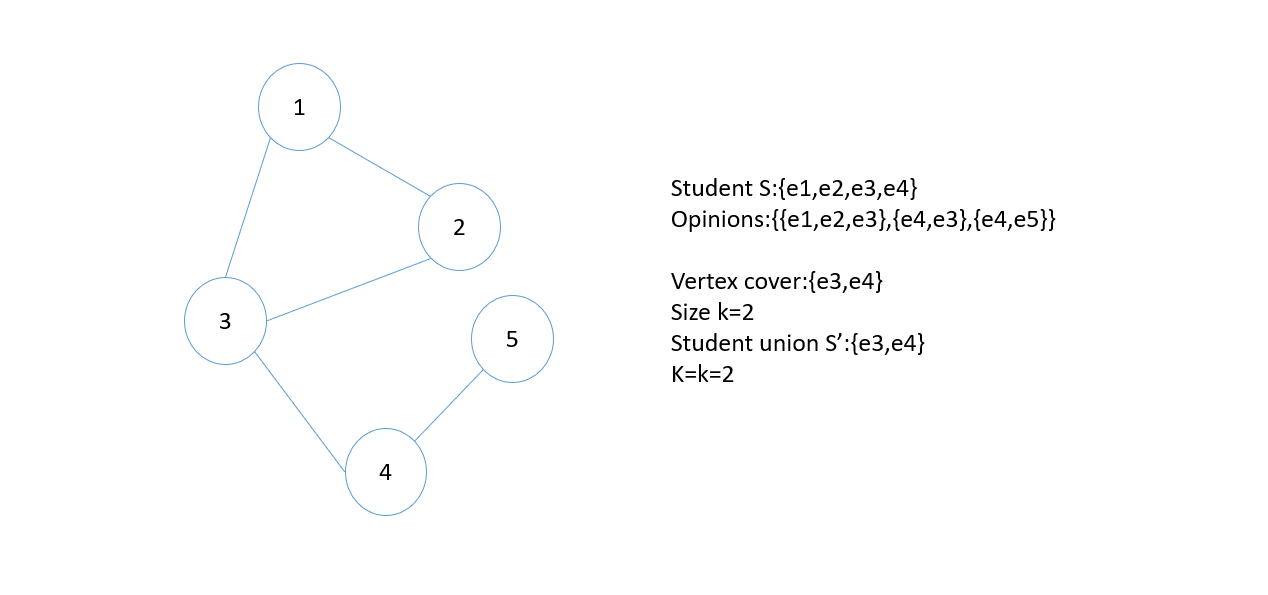
\includegraphics[width=0.9\textwidth]{2} 
		 
		\end{figure}

		Vertex-cover size $\le k$ iff $|S'|\le K$

		$\Rightarrow:$ For given vertex-cover, all vertex been covered represents that all complete graph is covered. Thus all opinions in ELECTION problem is covered. It's clear that $K=k$

		$\Leftarrow:$ For given instance of ELECTION, all opinions been covered all means all complete graph is covered. And the vertex size $k=K$.

		Therefore ELECTION problem is NP-complete.
	
	\end{proof}

	\item Not-All-Equal Satisfiability (NAE-SAT) is an extension of SAT where every clause has at least one true literal and at least one false one. NAE-$3$-SAT is the special case where each clause has exactly $3$ literals. Prove that NAE-$3$-SAT is NP-complete. (Hint : reduce $3$-SAT to NAE-$k$-SAT for some $k > 3$ at first)
	    \begin{proof}
	   First let's prove that 3-SAT can be reduced to NAE-4-SAT.
	   
	   For this we take an instance of 3-SAT and map each clause as follows:

	   $$(x\lor y\lor z)\rightarrow (x\lor y\lor z\lor s)\land (\lnot x\lor \lnot y\lor \lnot z\lor \lnot s)$$
	
	   For any assignment of SAT, there are  two cases. One is that the literals is not all equal and the two clauses of the NAE-4-SAT is also a valid assignment. Another is that $x,y,z$ are all true and a valid assignment of NAE-4-SAT is that $s$ is false.

	   For a assignment of NAE-4-SAT, if $s$ is true, we can simply invert the assignment to receive another valid assignment with $s$ isfalse. This is the assignment we want.
	
	   Thus $$3-SAT\le_pNAE-4-SAT$$

	   As a last step we reduce $NAE-4-SAT\le_pNAE-3-SAT$. 
	   
	   Take an instance in NAE-4-SAT and map the clauses as follows:

	   $$(a\lor b\lor c\lor d)\rightarrow (s\lor a\lor b)\land (\lnot s\lor c\lor d)$$

	   Notice here that if the true and false variable's (one of each must exist) are mapped to the same clause, s can be choose appropriately. If they are mapped to different clauses, s can be choose opposite to the respective variable value in each pair.

	   Thus $$NAE-4-SAT\le_pNAE-3-SAT$$

	   And NAE-3-SAT is easy to check in polynomial time.

	   Therefore NAE-3-SAT is NP-complete.
	\end{proof}

	\item In the Lab10, we have introduced Minimum Constraint Data Retrieval Problem (MCDR). Prove that MCDR (Version $1$ or $2$) is NP-complete. (Hint : reduce from VERTEX-COVER or $3$-SAT)
	    \begin{proof}
		
		First, we can certificate a MCDR instance by execute the download schedule and compute the switch times which equals the switch parameter, and compare it with bounded threshold k. It's obviously within polynomial time.

		Therefore, MCDR(version 1) is a NP problem.

		Next, We prove that $Vertex Cover\le_p MCDR$.

		Assume we have an instance of VERTEX-COVER problem: $G(V,E)$ and the cover set is $VC$. We can construct an instance of MCDR in the following ways.

		Every vertices in $G$ represents a channel and the number of channel is $|V|$.

		Every edge $e_{i,j}$ represents a data item $d_{i,j}$. And it was put on the channel $c_i$ and $c_j$ without gap and repeat non-stop so that every channel can switch to any another channel.

		After this construction, we prove that the vertex size $|VC|\le k$ iff $h\le k-1$ in MCDR instance.

		$\Rightarrow:$ For an instance of VERTEX COVER, we select all the cover vertices and they represent the needed data itmes in MCDR. Thus all request is satisfied. Because the size of $VC$ represents the switch times in MCDR, we can find a schedule with $|VC|-1$ switchs.

		$\Leftarrow:$ For given schedule of downloading data items, it need to switch to download different data items. Correspondingly, all data items been downloaded represents all vertices been covered and the size of $VC$ is $h+1$.

		Therefore MCDR problem(version 1) is NP-complete. 
	
		
	\end{proof}

\end{enumerate}

\textbf{Remark:} Please include your .pdf, .tex files for uploading with standard file names.




%========================================================================
\end{document}
